\section{Unblinding results}

This search for a new dark boson is done blindly to ensure that no bias is introduced in the
course of the analysis.
The data is unblinded in stages to ensure that the selection is behaving as expected on real data.

%Before any unblinding, the selection is checked using selected candidates
%consistent with the decay \decay{\Bd}{\jpsi\Kstarz}.
%The selection applied in the \sm analysis of \btokstrmumu, as described in
%\Ref{LHCb-CONF-2015-002}, yields $320\,000$ candidate decays.
%Using the selection from \Sect{sec:db:sel} and approximately \approx$260\,000$
%\decay{\Bd}{\jpsi\Kstarz} candidates remain.
%Therefore only \approx$10\%$ fewer events in this selection, which is not surprising
%considering this search is for a much rarer process than \decay{\Bd}{\Kstarz\mumu} in the \sm, and
%therefore selection requirements are likely to be tighter.

Selected \decay{\Bd}{\jpsi\Kstarz} events are used to check that the selection was not biased
based on neither the year, nor the polarity of the \lhcb magnet.
No bias is observed; in fact
efficiencies for the \uBDT are observed to be consistent to the $10^{-4}$ level in all four regions.

The unblinding procedure begins by checking the yield of the normalisation channel
\btokstrmumu in the range $1.1<\qsq<6.0\gevgev$ and comparing it with the yield from
\added{\Ref{LHCb-CONF-2015-002}, which details an angular analysis of this decay}.
The yield is taken from an unbinned fit to selected prompt \btokstrdb candidates using a mass model
of two Gaussian functions sharing the same mean, and with a power-law tail on the low mass side.
%same fit model for the signal component as used in \Ref{LHCb-CONF-2015-002}, which is the sum of
A simple exponential models the background component.
This yields 527 \Bd candidates, which can be compared to \approx$625$ events in the \sm selection,
where the drop in signal is, again, expected given the search is for a rare process.
Together with the drop in signal, comes a drop in background yield, from \approx$630$ background
events over the full mass range, to only 290.
Figure~\ref{fig:db:norm} shows the \Bd candidate mass spectrum for the normalisation channel, and
the fitted distribution overlaid.

\begin{figure}
  \begin{center}
    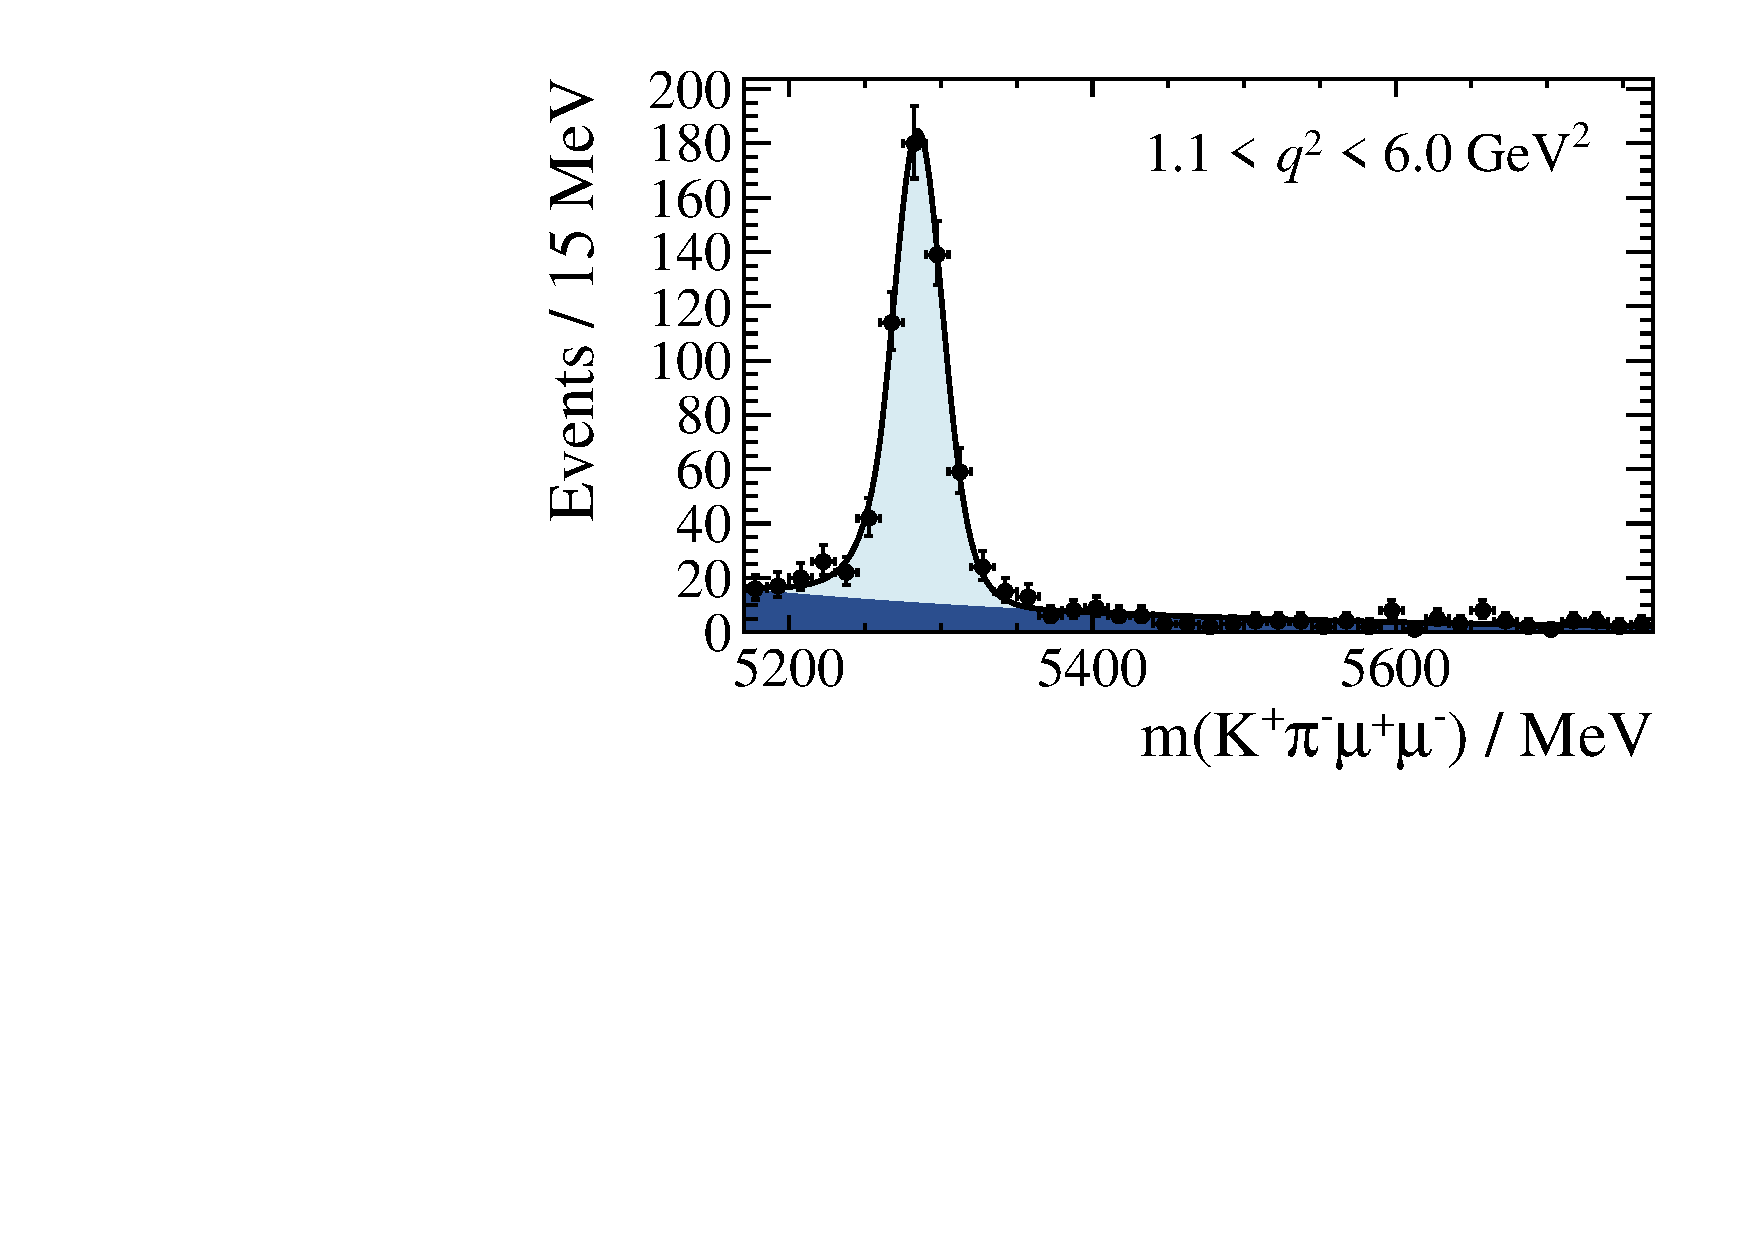
\includegraphics[width=0.6\textwidth]{norm_channel}
    \caption[Fit to the normalisation channel, \btokstrmumu for $1.1<\qsq<6.0\gevgev$]
    {
      Fit to the invariant mass spectrum of the \Bd candidates in selected data in the range
      $1.1<\qsq<6.0\gevgev$.
      The signal model is the sum of two Gaussian functions with power-law tails on the low-mass
      side with parameters taken from the analysis described in
      Ref.~\protect\cite{LHCb-CONF-2015-002},the background model is a decaying exponential.
      This fit results in a signal yield of $(527\pm26)$ compared to approximately 625 in the \sm
      analysis.
      %for more in depth numbers, please refer to Table~\protect\ref{tab:db:nums126}.
    }
    \label{fig:db:norm}
  \end{center}
\end{figure}

After unblinding the region $1.1<\qsq<6.0\gevgev$, other prompt \qsq regions were also used to
confirm that the ratio of \bdt selection efficiencies
$\varepsilon_\mathrm{BDT}^\mathrm{\qsq bin}(\btokstrmumu) / \varepsilon_\mathrm{BDT}(\btojpsikstr)$
are approximately the same in data and simulation.
To determine these efficiencies, the full selection without the \BDT is taken, and a fit performed
and the signal yield is extracted.
Next, the \BDT is applied and a second fit is performed, then \deleted{take} the ratio of the signal
yields \added{is calculated}.
A comparison between these numbers in data and simulation is shown in comparison is shown in
\Fig{fig:bdtEffRatio}; the two distributions are shown to be in good agreement, centred around
unity with about 5--10\% precision.
%This approach ignores the fact that there may be some small peaking background component that gets
%counted as signal pre-BDT cut, but is removed by the BDT.
%Note, however, that in the
%$\varepsilon_\mathrm{BDT}^\mathrm{\qsq bin} / \varepsilon_\mathrm{BDT}^{\decay{\Bd}{\jpsi\Kstarz}}$
%ratio, only the difference in peaking background contributions matters.
%Given that all peaking backgrounds that are visible in the various 2-body mass combinations are
%explicitly vetoed, no peaking background contributions at the level of the statistical precision of
%this test are expected.

\begin{figure}
  \begin{center}
    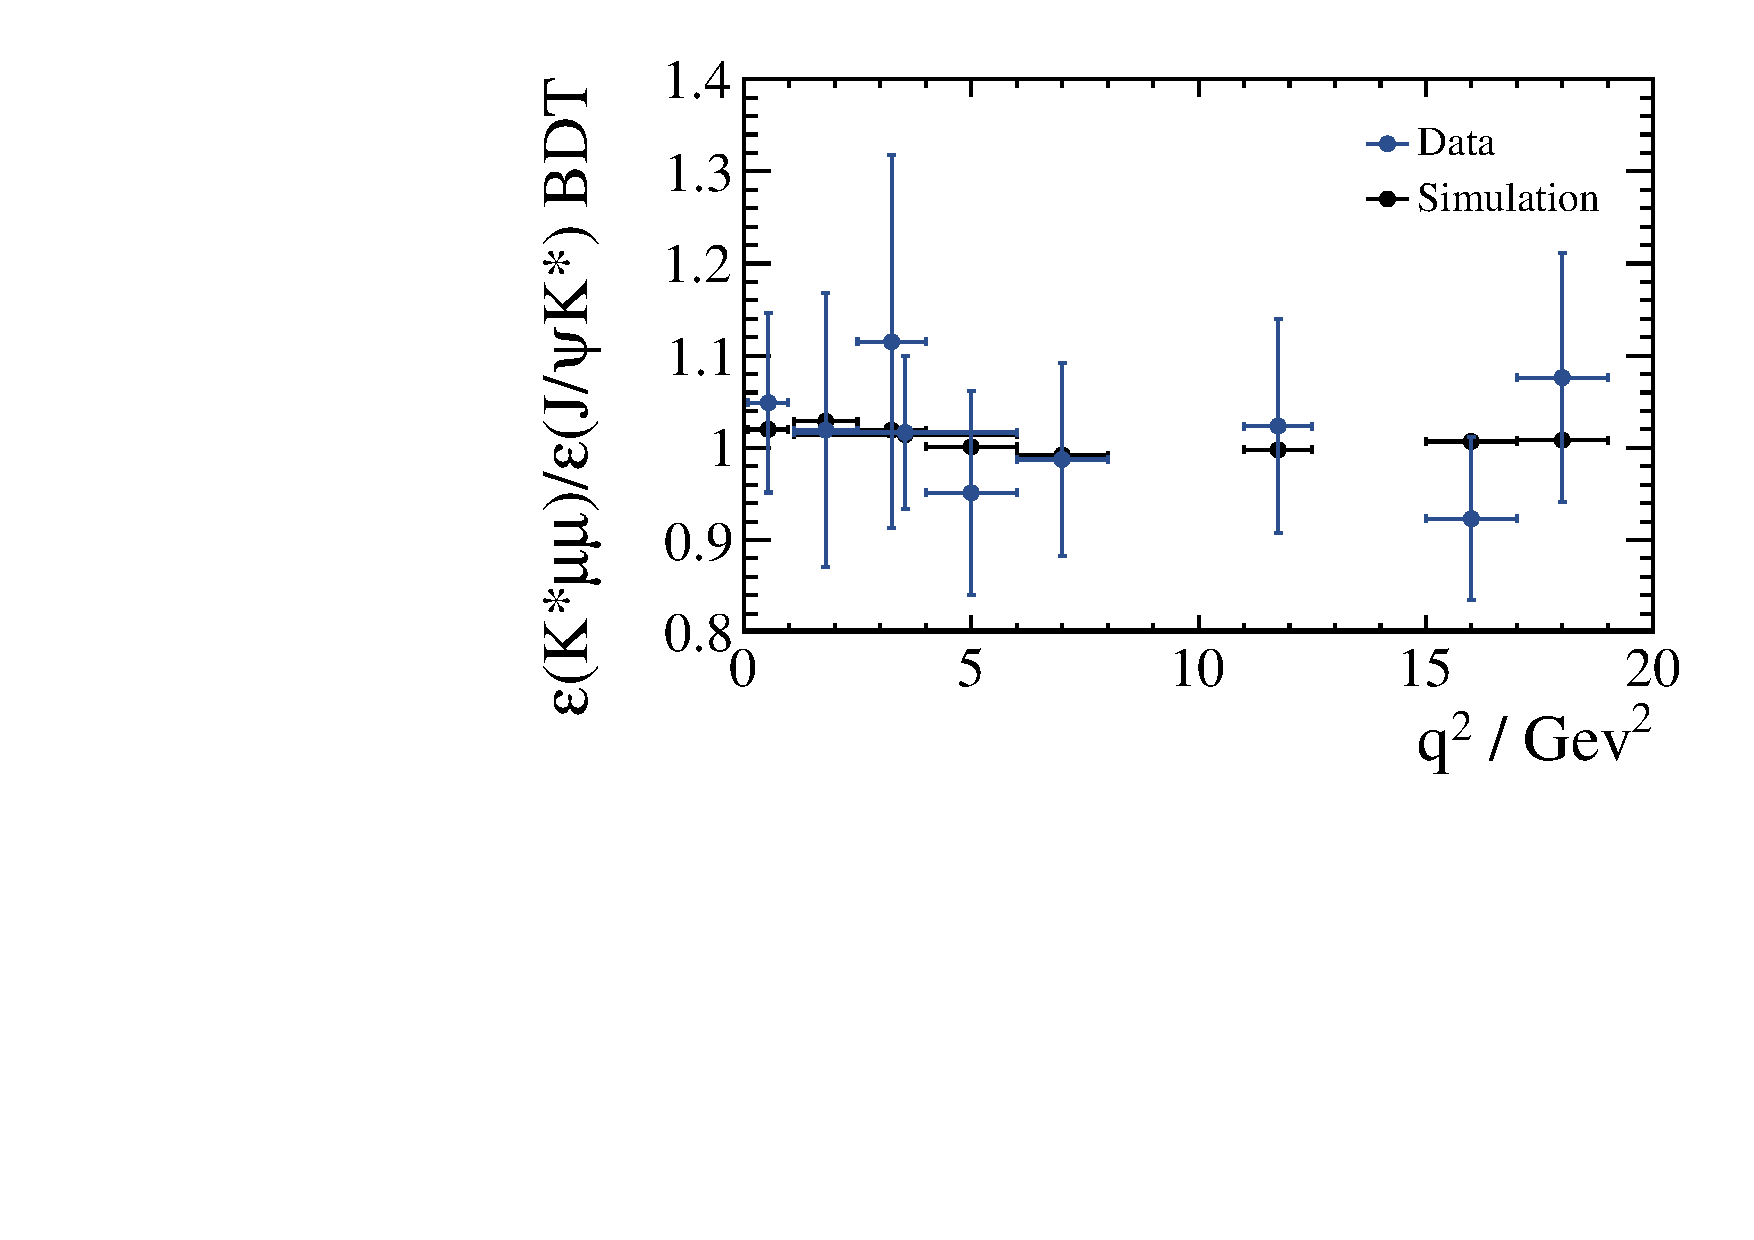
\includegraphics[width=0.48\textwidth]{bdtEffRatio}
    \caption[Efficiency ratios]
    {
      Ratio of the efficiencies of the \bdt selection for a range of \qsq bins, as used in the SM
      \btokstrmumu analysis, with respect to the efficiency for \decay{\Bd}{\jpsi\Kstarz}.
      Data and simulation are shown to be in good agreement.
    }
    \label{fig:bdtEffRatio}
  \end{center}
\end{figure}

Using the unblinded distributions it is possible to estimate the amount of combinatorial background
that will remain in the final selection.
Fitting an exponential to model the background across the signal region allows an approximate
number of events in the combinatorial background to be deduced.
This number of events can be taken from the upper-mass sideband, and the invariant mass of the
dimuon pair can be plotted.
With this method, it expected that a maximum of 10(2) events will contribute to the background in
the prompt(displaced) region at a single test mass, but on average the value is 1.8(0.2) events per
bin.
Figure~\ref{fig:db:comb} shows the shape and scale of the combinatorial background, and the fits
used to calculate it.

\begin{figure}
  \begin{center}
    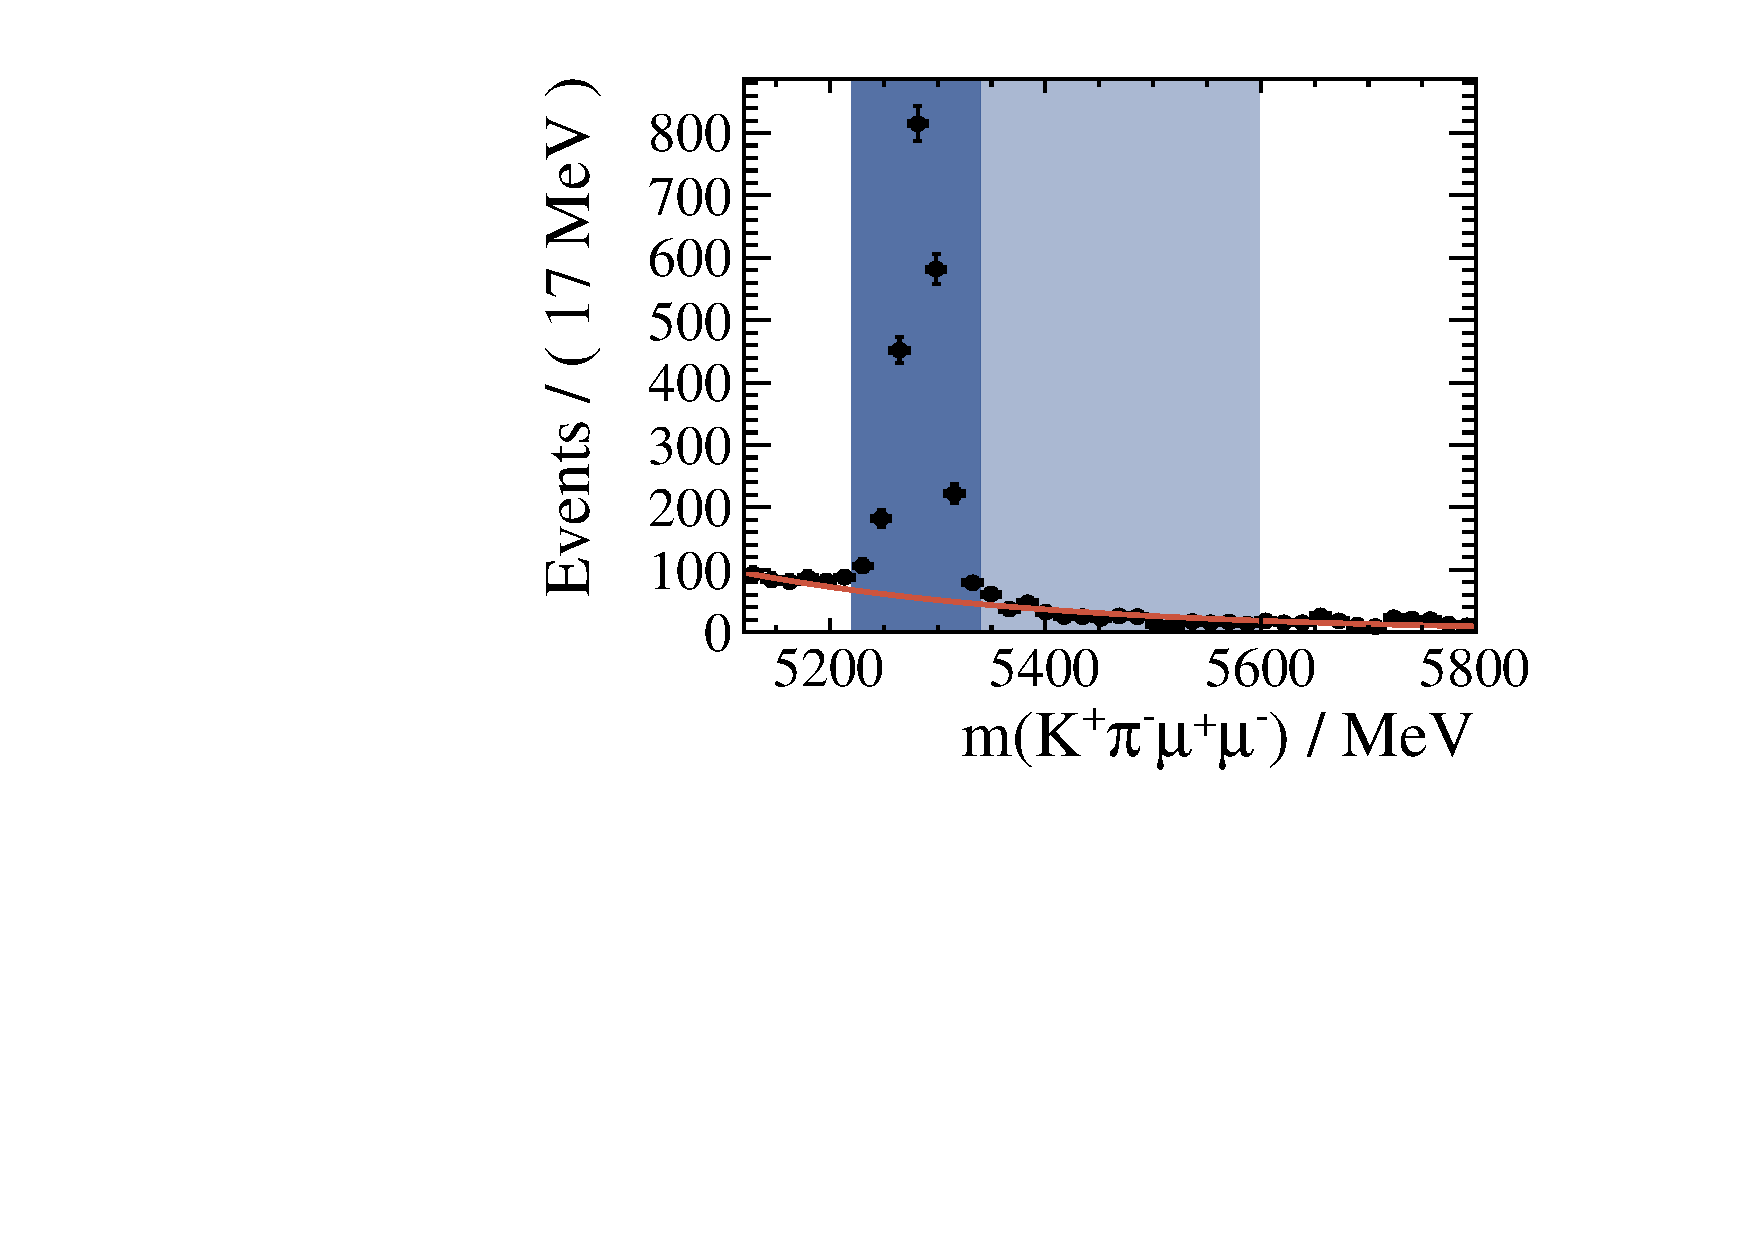
\includegraphics[width=0.48\textwidth]{combinatorial_prompt_fit}
    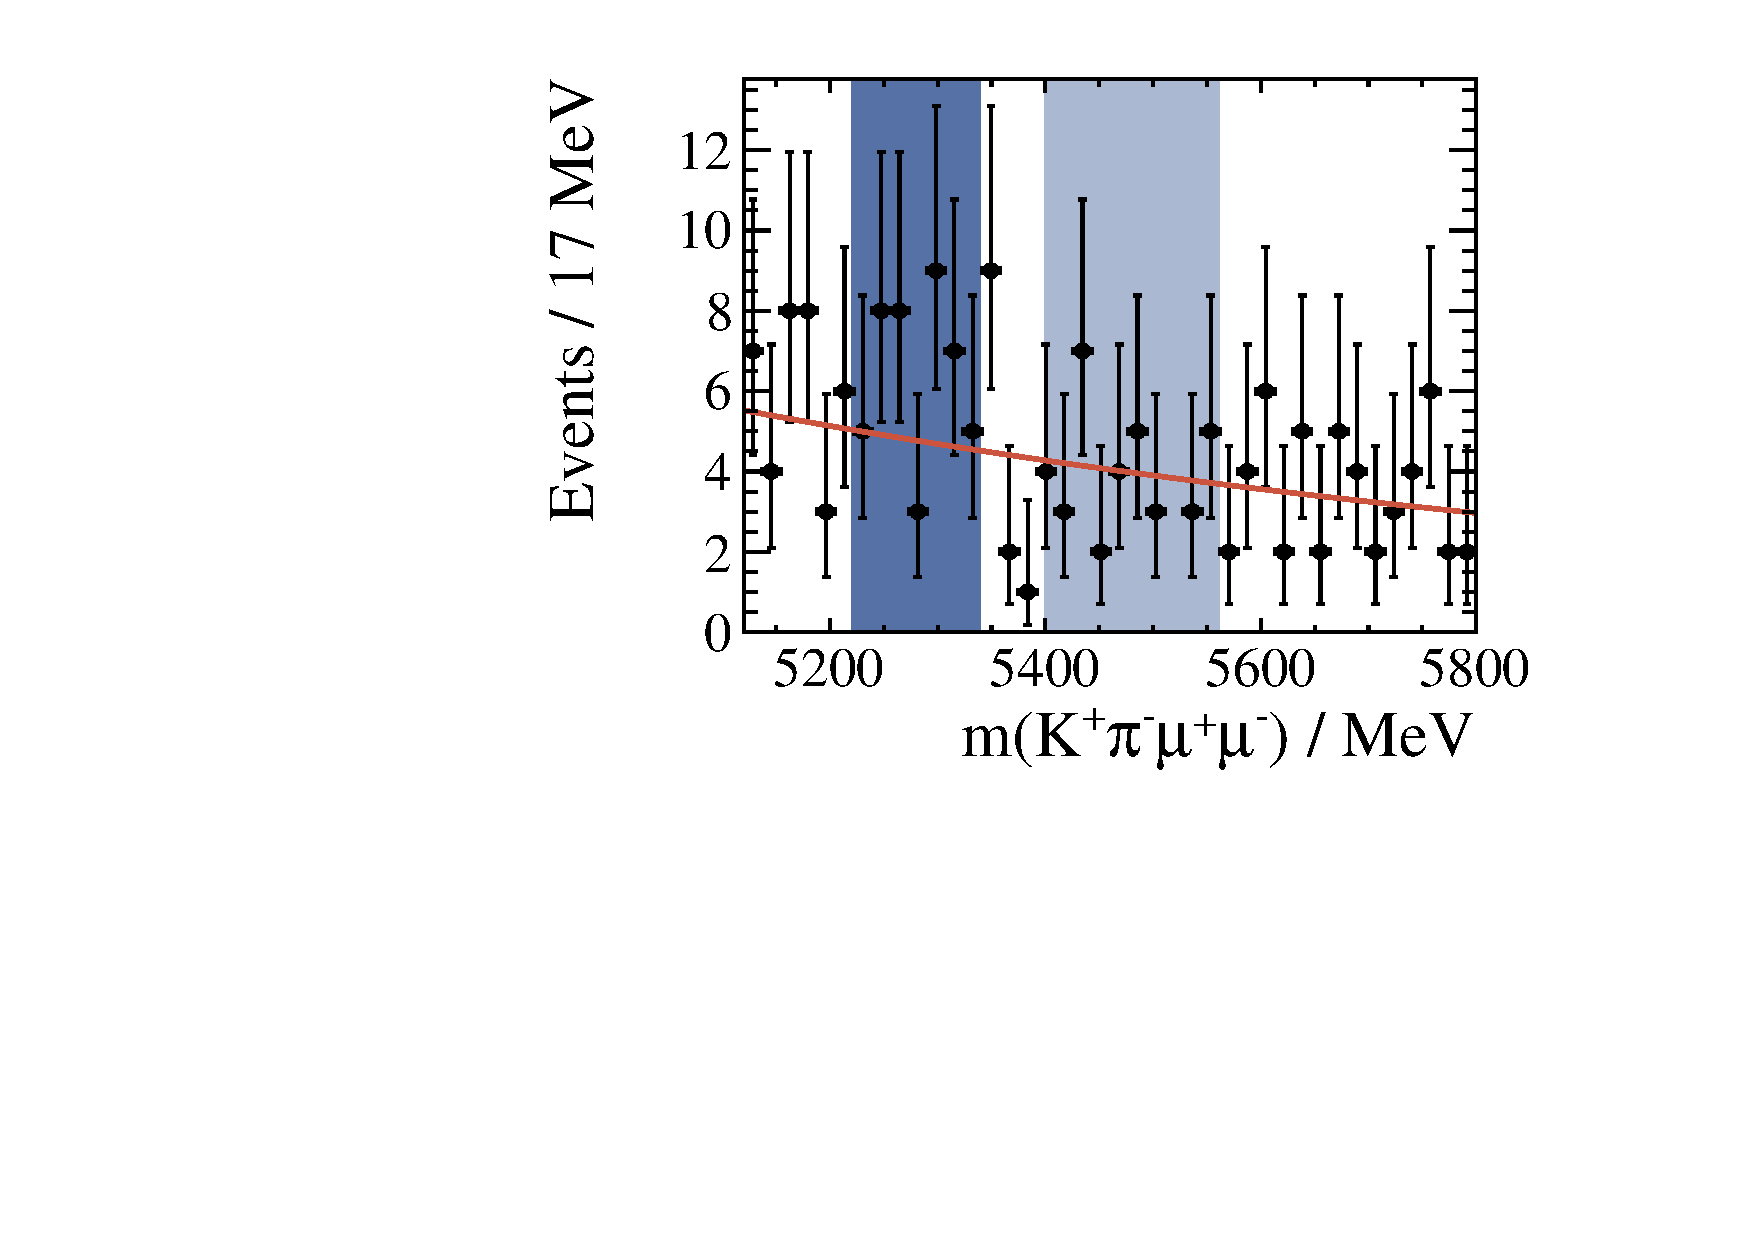
\includegraphics[width=0.48\textwidth]{combinatorial_displaced_fit}
    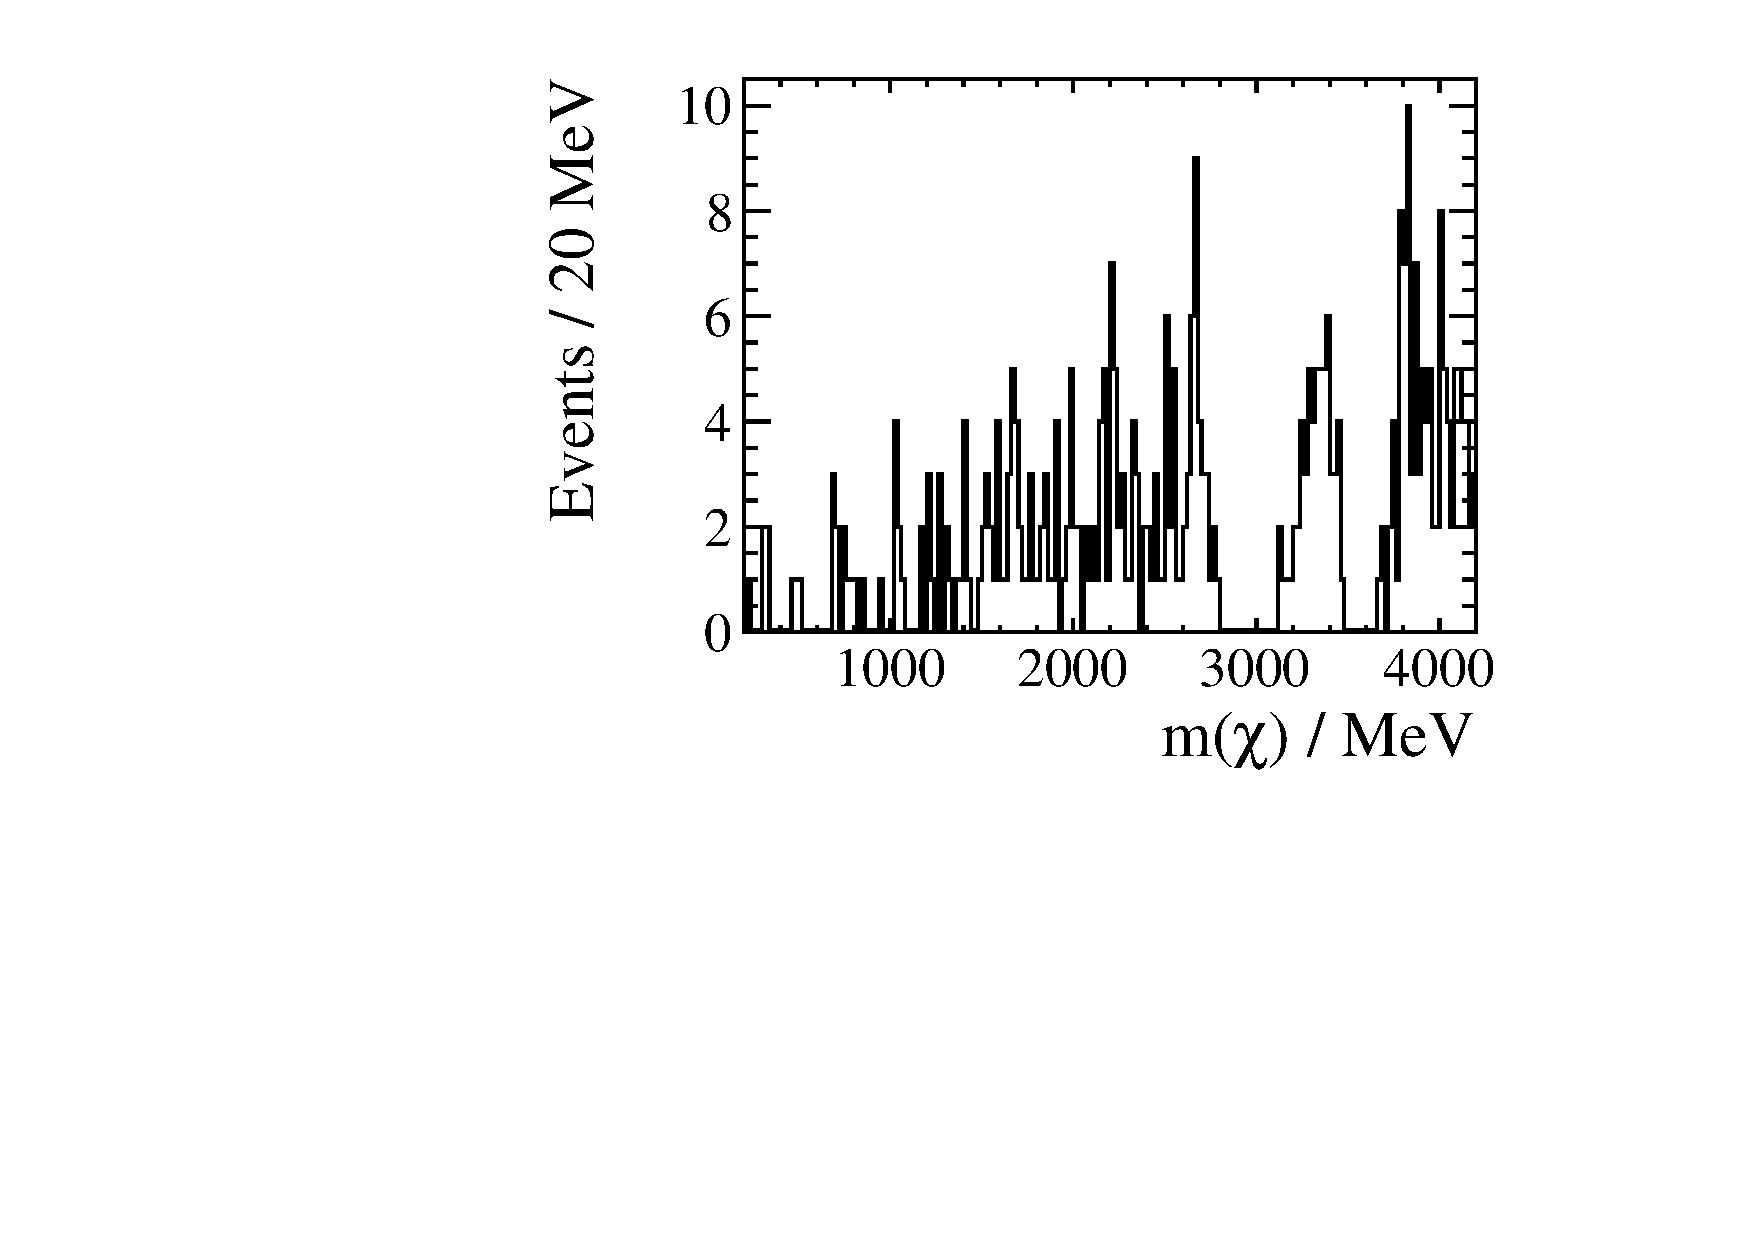
\includegraphics[width=0.48\textwidth]{combinatorial_prompt}
    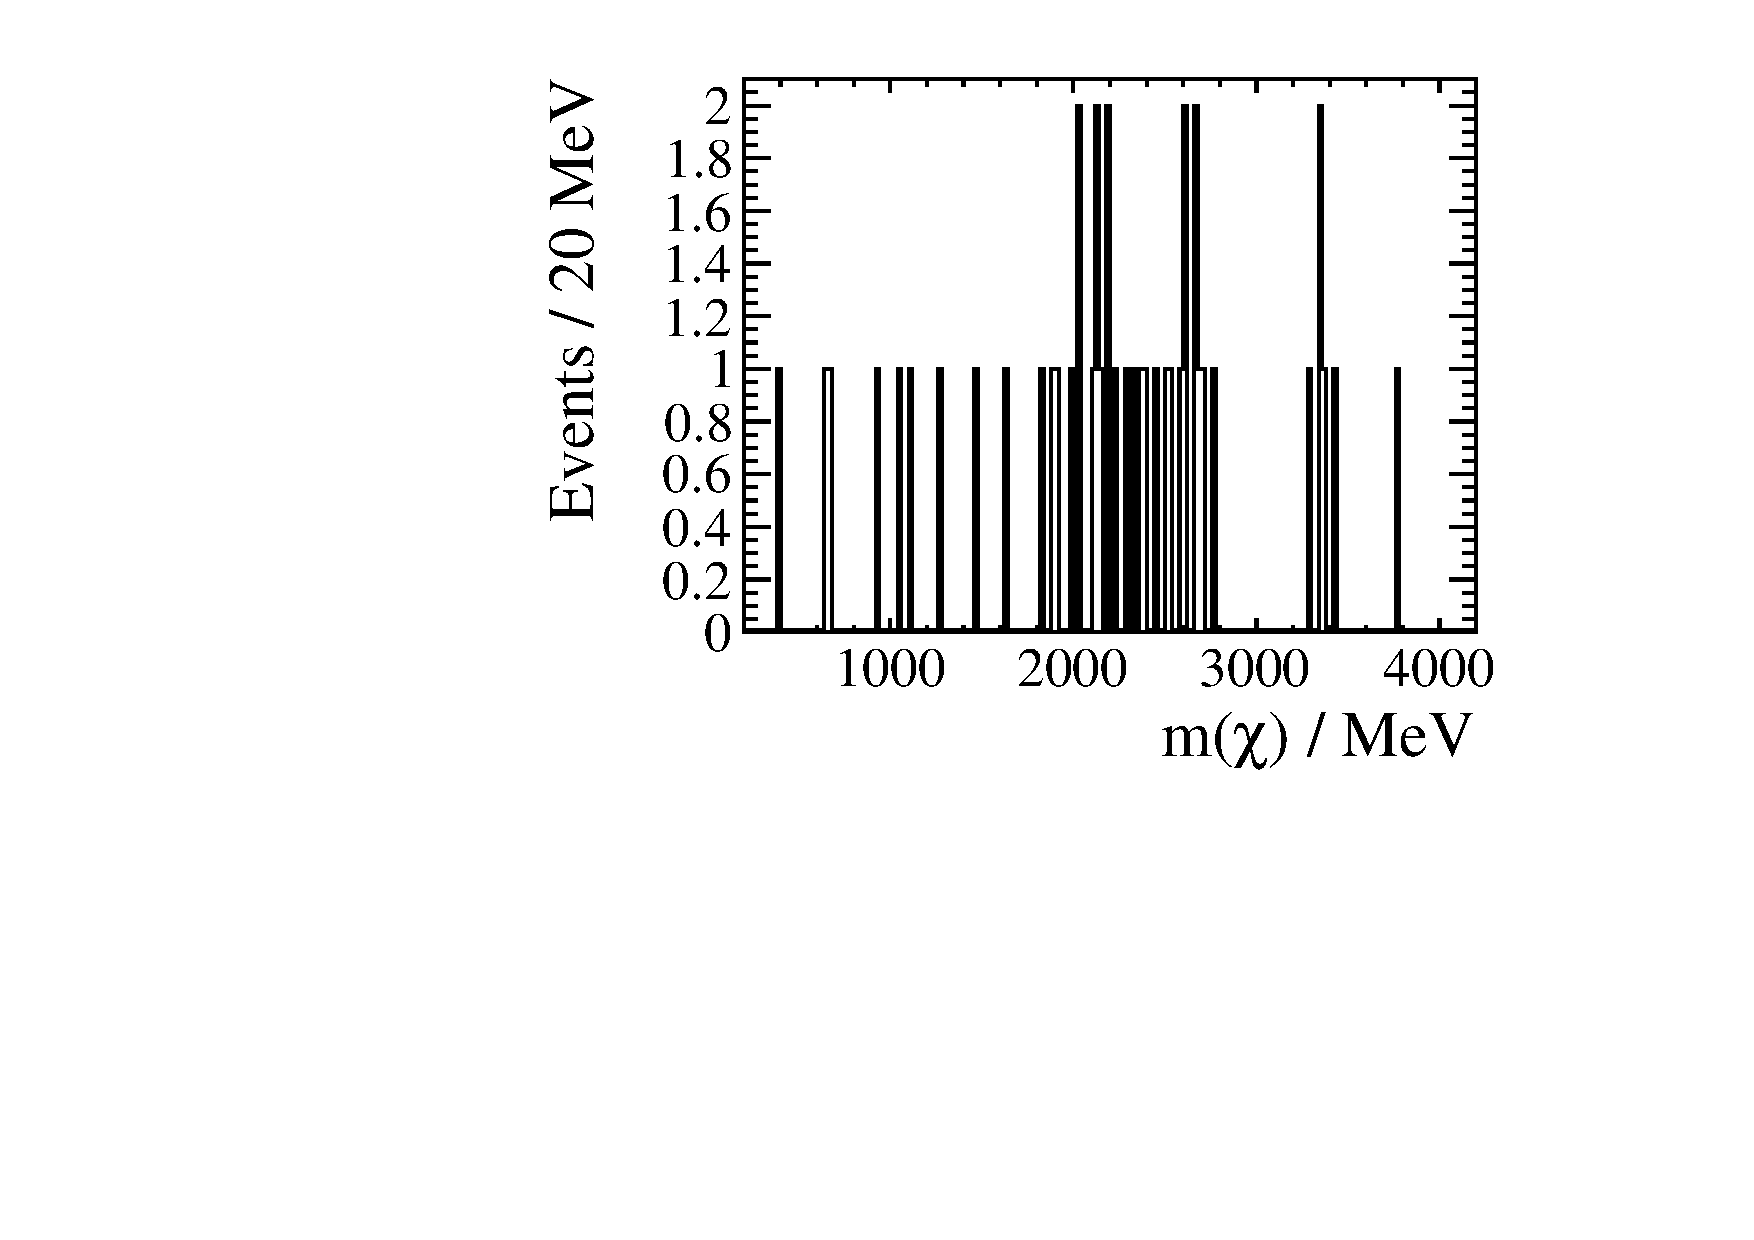
\includegraphics[width=0.48\textwidth]{combinatorial_displaced}
    \caption[Estimation of combinatorial background contribution]
    {
      Fits to the background component of selected \btokstrmumu events are shown in the upper
      plots, where the dark blue regions are not used in the fit, but are used to determine the
      number of events contributing to the combinatorial background by integrating across the
      region.
      The light blue region covers the same number of background events as in the darker region;
      these are purely combinatorial background, and the invariant dimuon masses are plotted below,
      using a bin width that is approximately equal to the width of the signal region in where the
      mass resolution is at its worst.
    }
    \label{fig:db:comb}
  \end{center}
\end{figure}



%At the time of writing, the unblinding procedure is no further than indicated above.
%As time progresses the whole dataset will be unblinded.
%First in binned distributions
%--- which will hide any potential signal, assuming the signal is not extremely obvious ---
%in the prompt and displaced regions.
%From these distributions toy datasets can be generated and used to convert the local minimum
%$p$-value to a global one, the procedure for which is described in \Sect{sec:db:strategy}.
%Systematic uncertainties will be evaluated and upper limits will be set for a range of \mass{\db}
%and \lifetime{\db}.

\subsection[Calculation of the $p$-value]
{Calculation of the $\boldsymbol{p}$-value}

The unblinded distribution in $m_{\mumu}$ is shown in \Fig{fig:db:mumu}.
Using the statistical method described in \Sect{sec:db:strategy} the following ranges in \mass{t}
are scanned:
\begin{align*}
  253.4 &< \mass{t} < \pz369.5 \mev, \\
  574.5 &< \mass{t} < \pz906.5 \mev, \\
  1136.0 &< \mass{t} < 2813.0 \mev, \\
  3246.5 &< \mass{t} < 3576.5 \mev, \\
  3796.0 &< \mass{t} < 4356.0 \mev.
\end{align*}
Values of \mass{t} do not reach threshold boundaries because of the sidebands extending in either
direction.
The minimum local $p$-value is found to be $3.6\e{-3}$ at $m_{t}^\mathrm{min} = 4285.0\mev$.

The look-elsewhere effect must be considered.
To convert the $p$-value to a global one, a \PDF is fit to the \mass{\mumu} distribution of the
prompt and displaced \btokstrdb candidates that lie outside of the vetoed regions, and outside of
the signal region centred at $m_t^\mathrm{min}$.
A fourth(second) order Chebychev polynomial is fit to candidates in the prompt(displaced) region.
From these \glspl{PDF} $1.5\e{7}$ toy datasets are generated, and the minimum $p$-value for each
one is calculated.
Constructing a cumulative distribution of these $p$-values makes an easy conversion from local to
global $p$-values, this conversion is shown in \Fig{fig:db:mumu}.
Shown alongside the cumulative histogram is the asymptotic approximation, which is seen to be in
excellent agreement for local $p$-values less than about $10^{-4}$.
The histogram converts the local $p$-value to a global $p$-value of $0.63$, equivalent to a shift
in significance of $2.9\stdev$ to $0.63\stdev$.
These results show no evidence for a new dark boson in the mass ranges given above.

\begin{figure}
  \begin{center}
    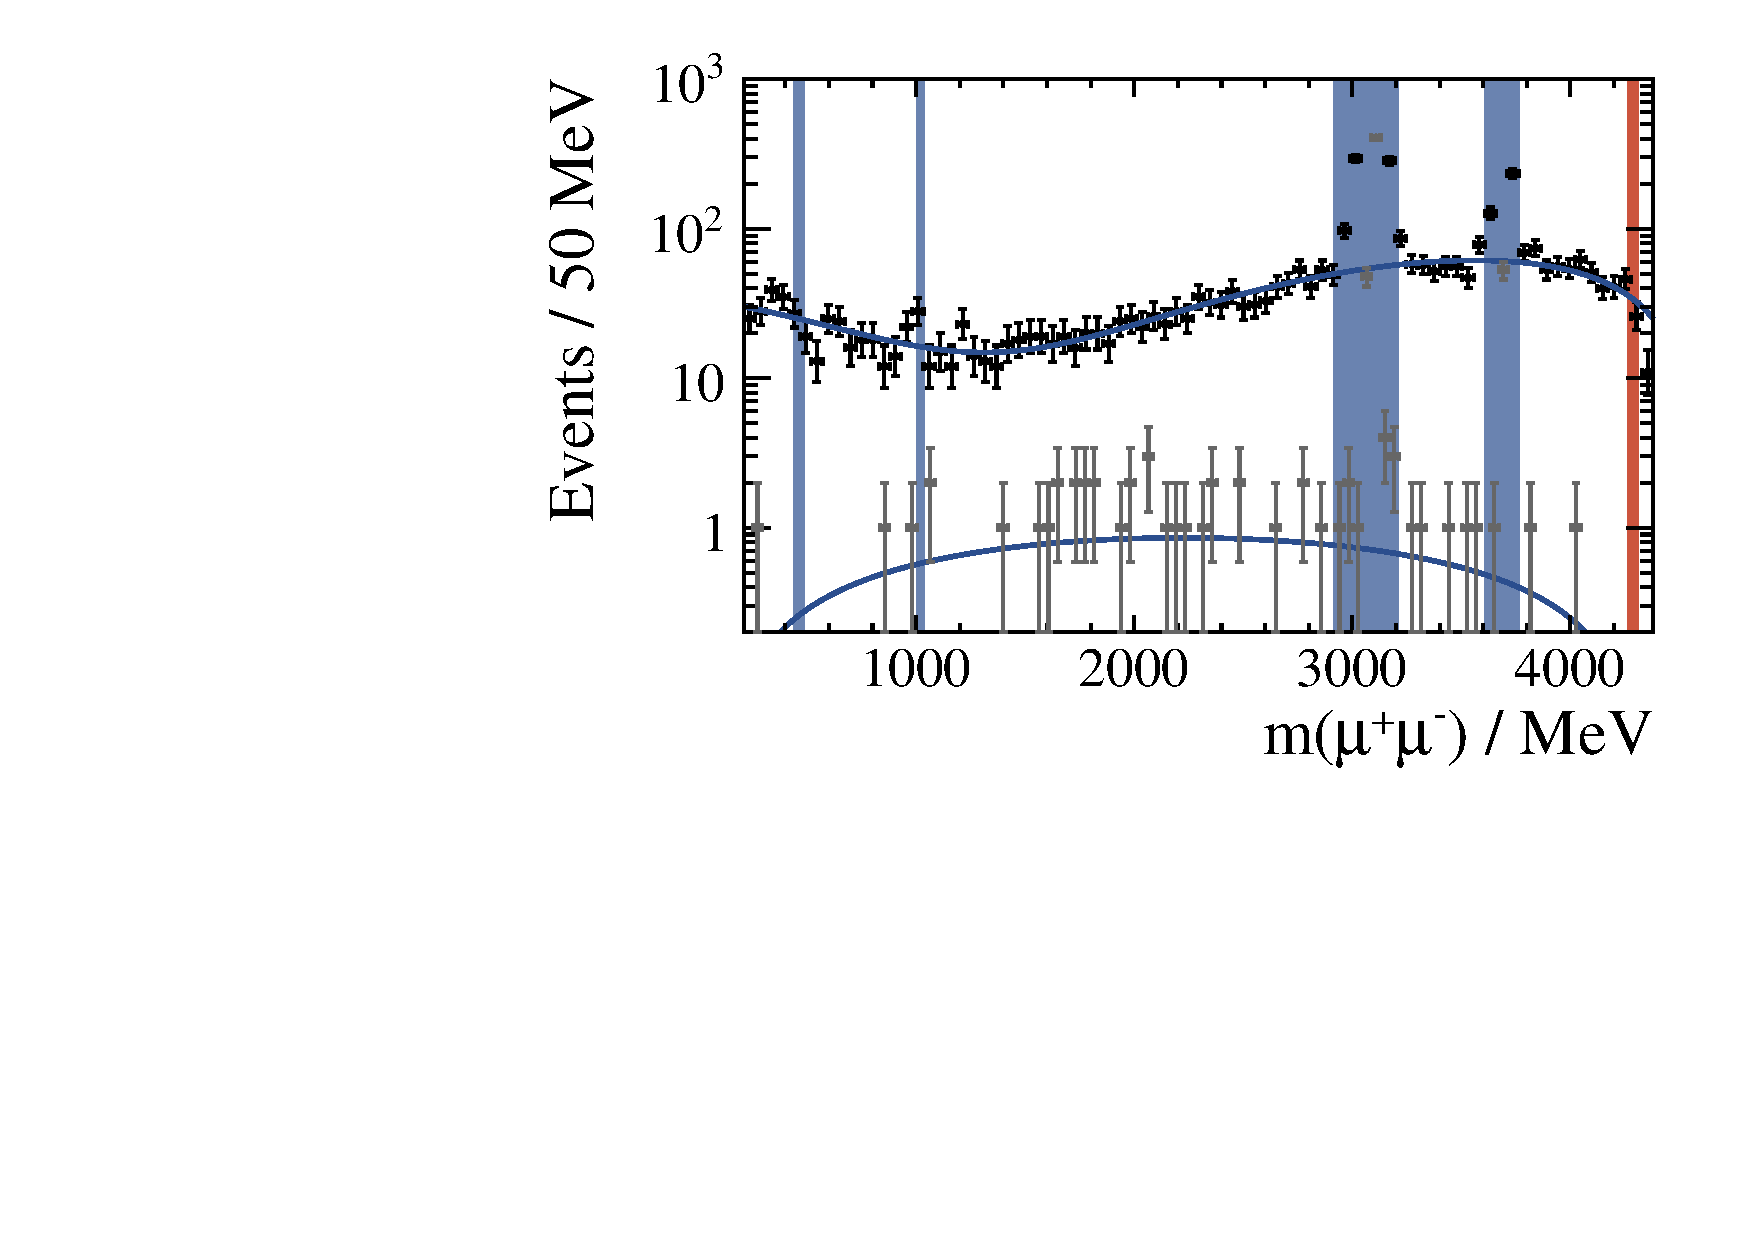
\includegraphics[width=0.48\textwidth]{mxpdf}
    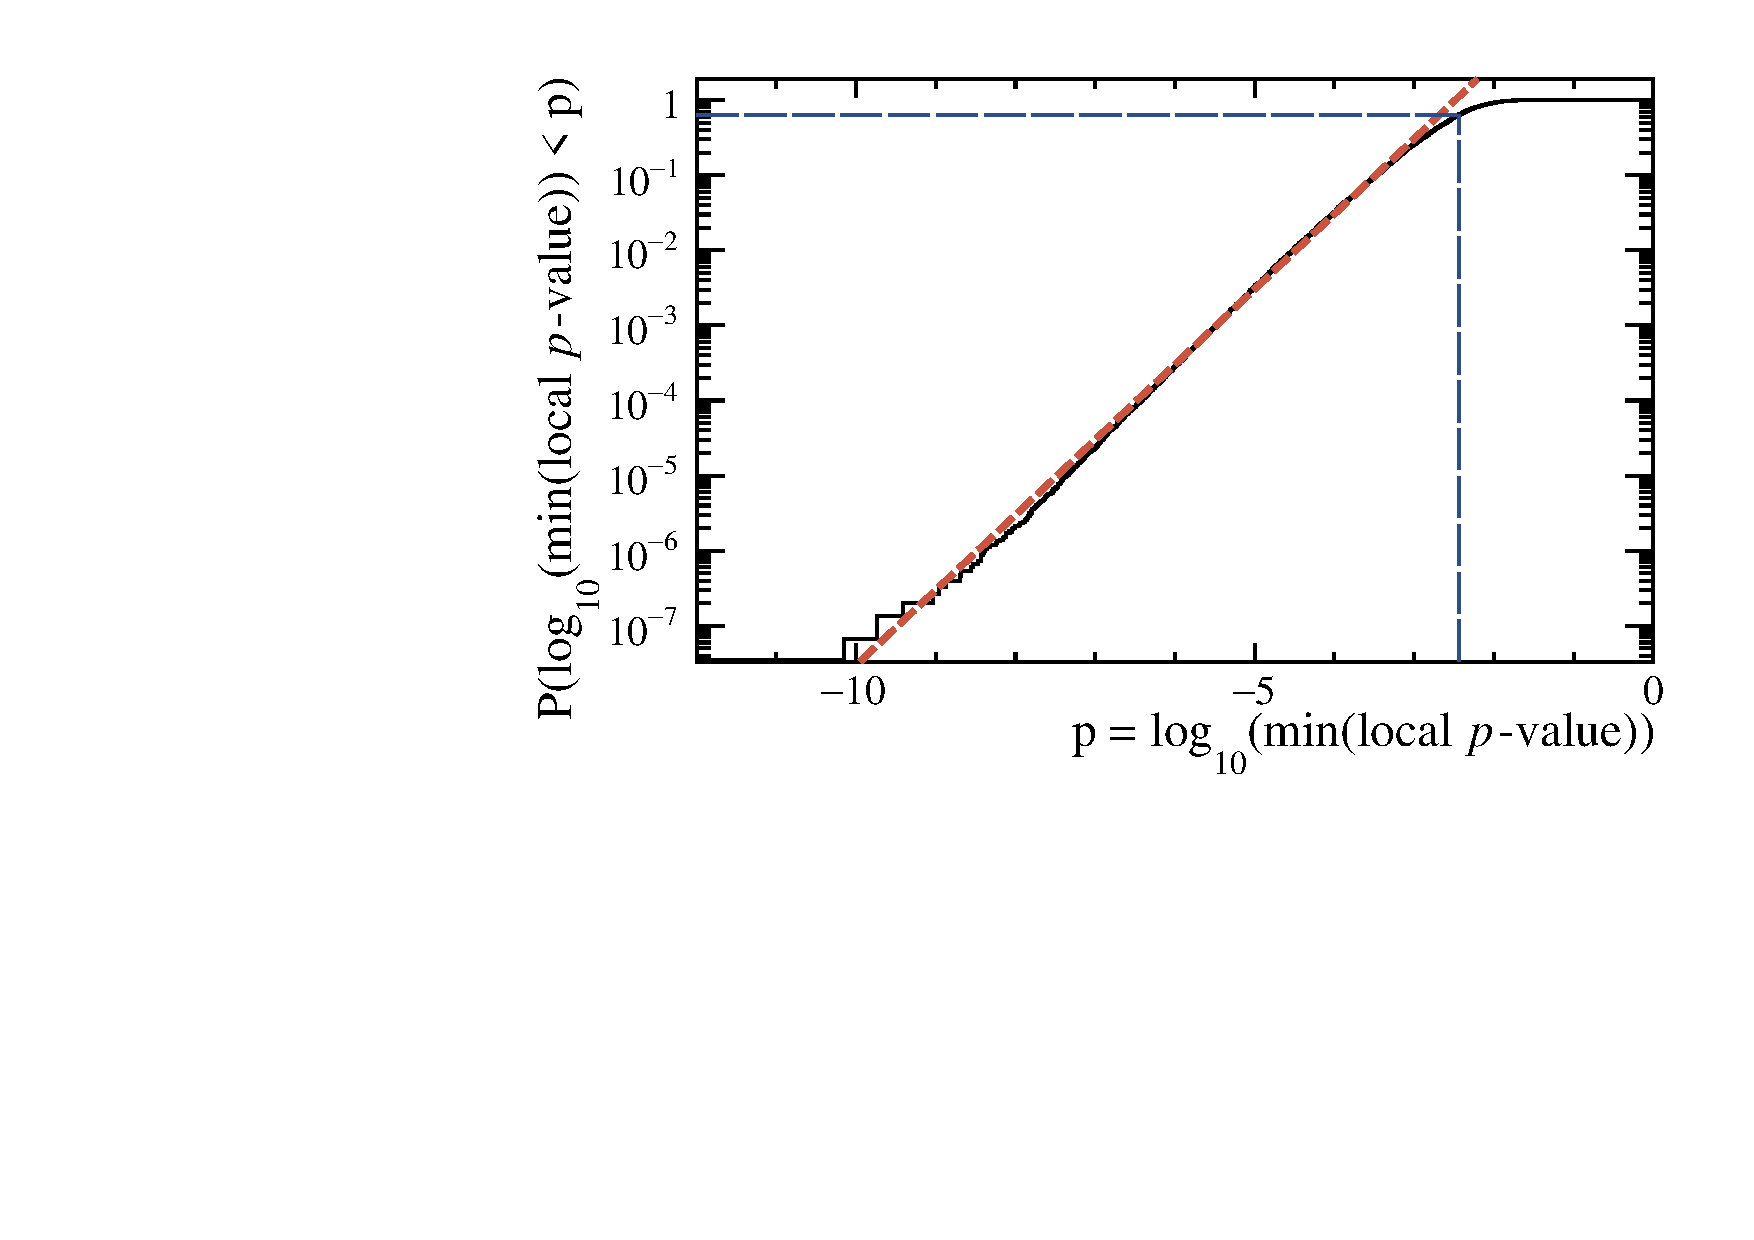
\includegraphics[width=0.48\textwidth]{pvalConversion}
    \caption[dimuon mass distribution and $p$-value calculation]
    {
      Invariant mass distributions of the dimuon pair are shown on the left, while
      prompt and displaced candidates are black and grey points, respectively.
      Chebychev polynomials fitted to the data are shown as solid blue lines.
      The narrow red region indicates $|m_{t}-4285.0|<5\sigmam$ ($x=1$ in this region).
      On the right is the result of running the method on $1.5\e{-7}$ toy datasets, used to convert
      the local $p$-value ($3.6\e{-3}$) to a global one (0.63). This conversion is indicated by the
      blue dashed line.
      The result of the asymptotic formula is shown by the red dashed line, and is seen to be an
      excellent approximation of the true distribution.
    }
    \label{fig:db:mumu}
  \end{center}
\end{figure}

%253.4 -> 369.5
%574.5 -> 906.5
%1136 -> 2813
%3246.5 -> 3576.5
%3796 -> 4356
%3.610859e-03,  4285.035MeV => 2.9sigma
%0.63322 => 0.48sigma global
% RooStats::PValueTOSignificance(pval / 2)



\subsection{Systematic uncertainties}
Systematic uncertainties must be assessed in order to set limits.
Sources of systematic uncertainties are from:
the ratio of efficiencies $\varepsilon(\btokstrdb)/\varepsilon(\btokstrmumu)$;
the of prompt and displaced regions as defined by the lifetime resolution;
and the uncertainty on the \btokstrmumu branching fraction in the range $1.0<\qsq<6.0\gevgev$.
\added{
These systematic uncertainties do not have any effect on the significance level of the minimum
local $p$-value.
}

\added{
In the prompt region the efficiency ratio $\eff{\Bd\!\to\Kstarz\db(\mumu)}/\eff{\btokstrmumu}$ is
constructed to be close to unity, and should be preserved by the selection for all lifetimes.
This preservation is validated by comparing \decay{\Bd}{\jpsi\KS} in data and simulation.
The full selection, including the \uBDT where the $\ProbNN{\mu}$ input is replaced by
$\ProbNN{\pi}$,
is applied, using the \KS as a proxy for the \db.
Mass cuts are also applied to isolated the \jpsi and \KS candidates,
and a cut of $\lifetime{\KS}>0.2\ps$ is applied to avoid prompt
backgrounds such as \decay{\Bd}{\jpsi\pipi}.
Lifetime distributions for these selected \KS candidates in data and simulation are shown in
\Fig{fig:db:syst:effrat}.
These distributions would be approximately uniform without detector effects; the degree to which
the distributions agree demonstrates that the simulation models the detector well, and results in a
negligible systematic uncertainty.
}


\begin{figure}
  \begin{center}
    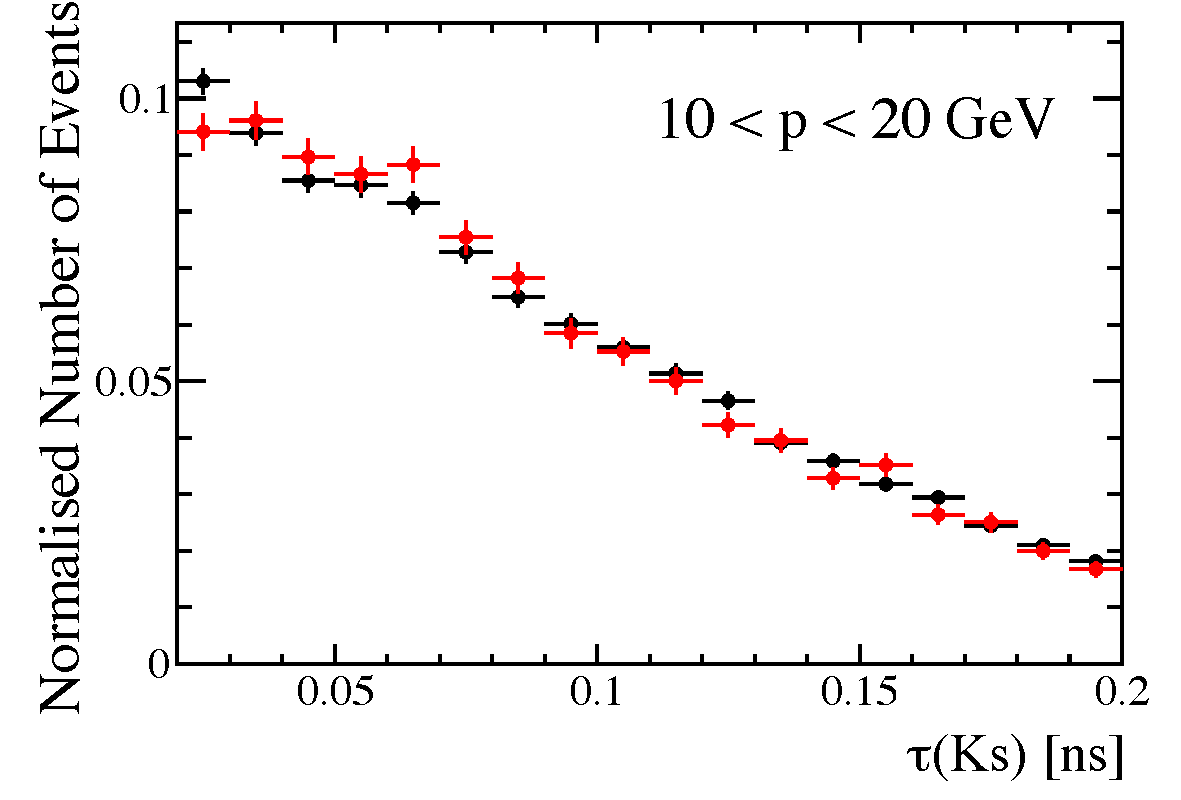
\includegraphics[width=0.48\textwidth]{jks_0}
    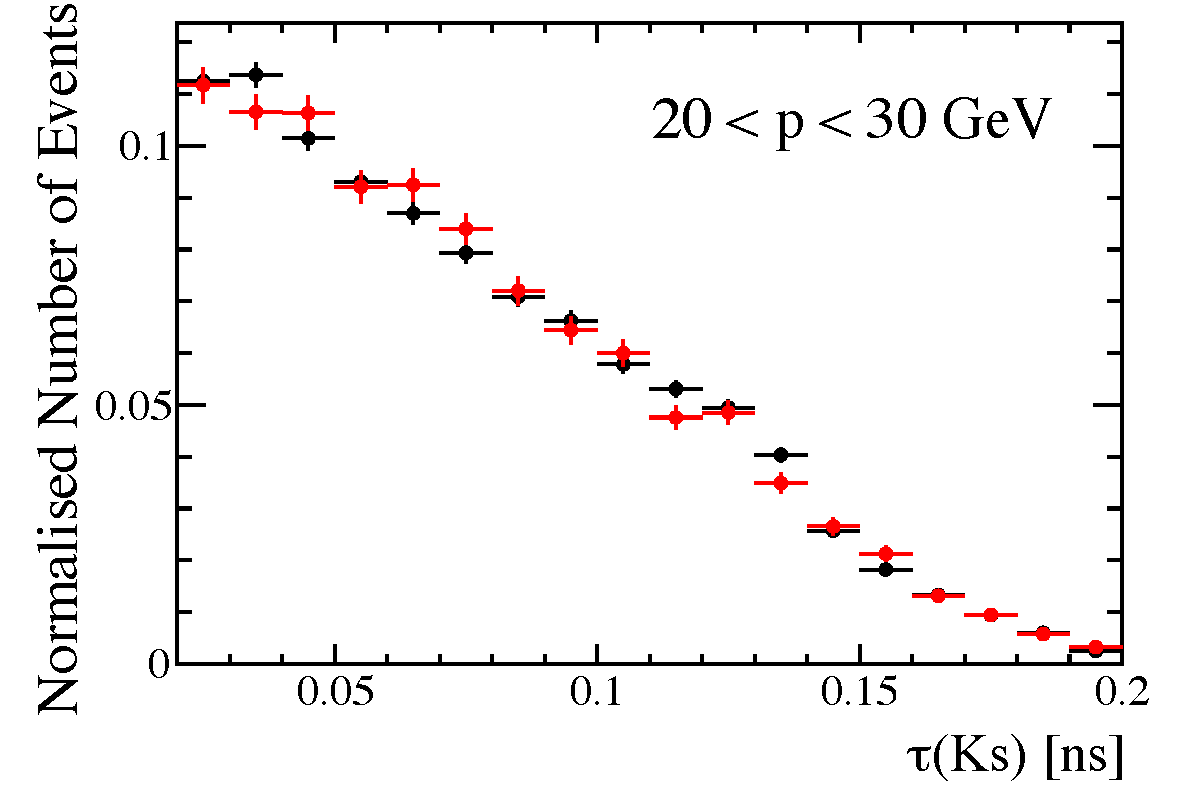
\includegraphics[width=0.48\textwidth]{jks_1}\\
    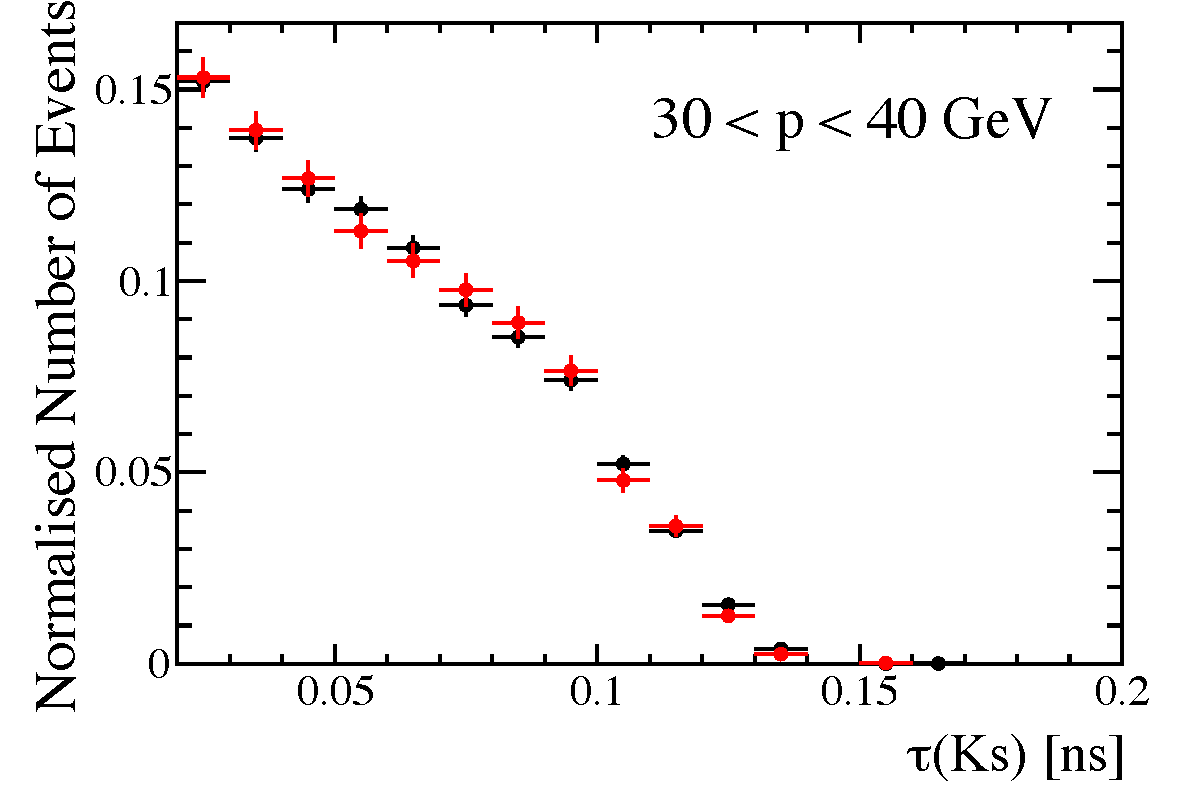
\includegraphics[width=0.48\textwidth]{jks_2}
    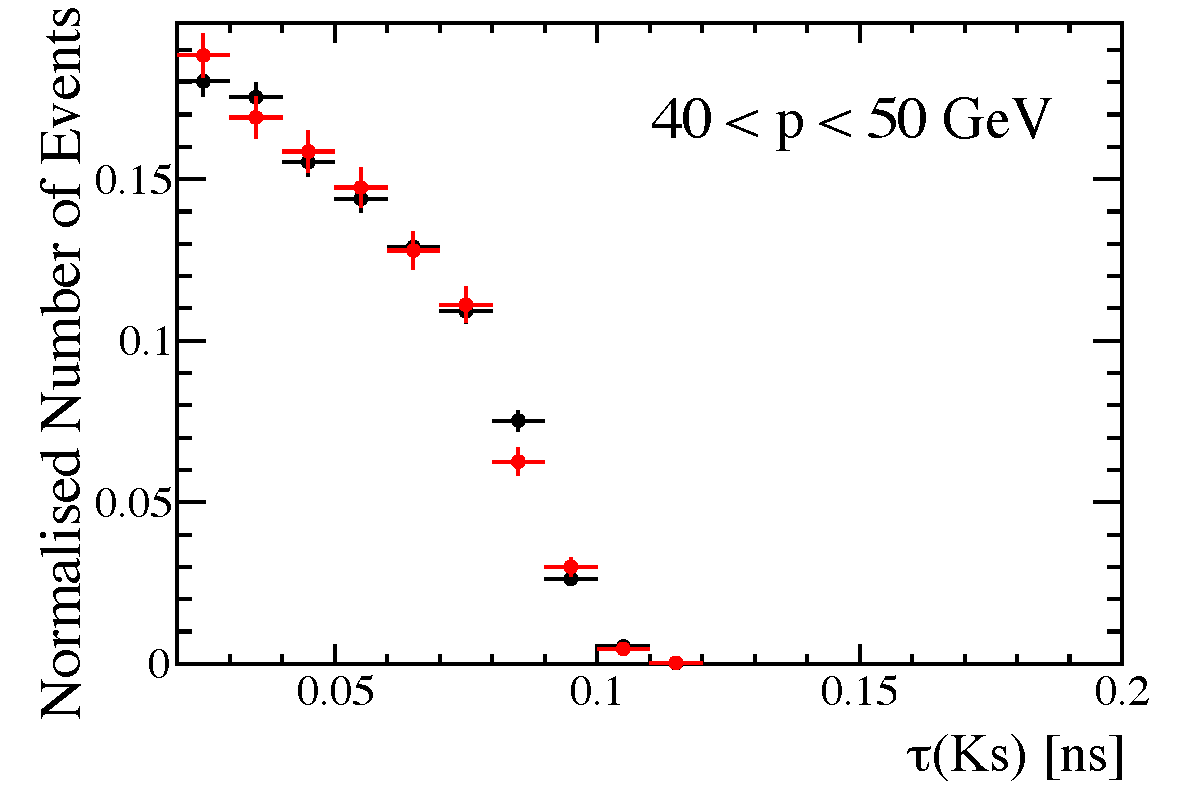
\includegraphics[width=0.48\textwidth]{jks_3}\\
    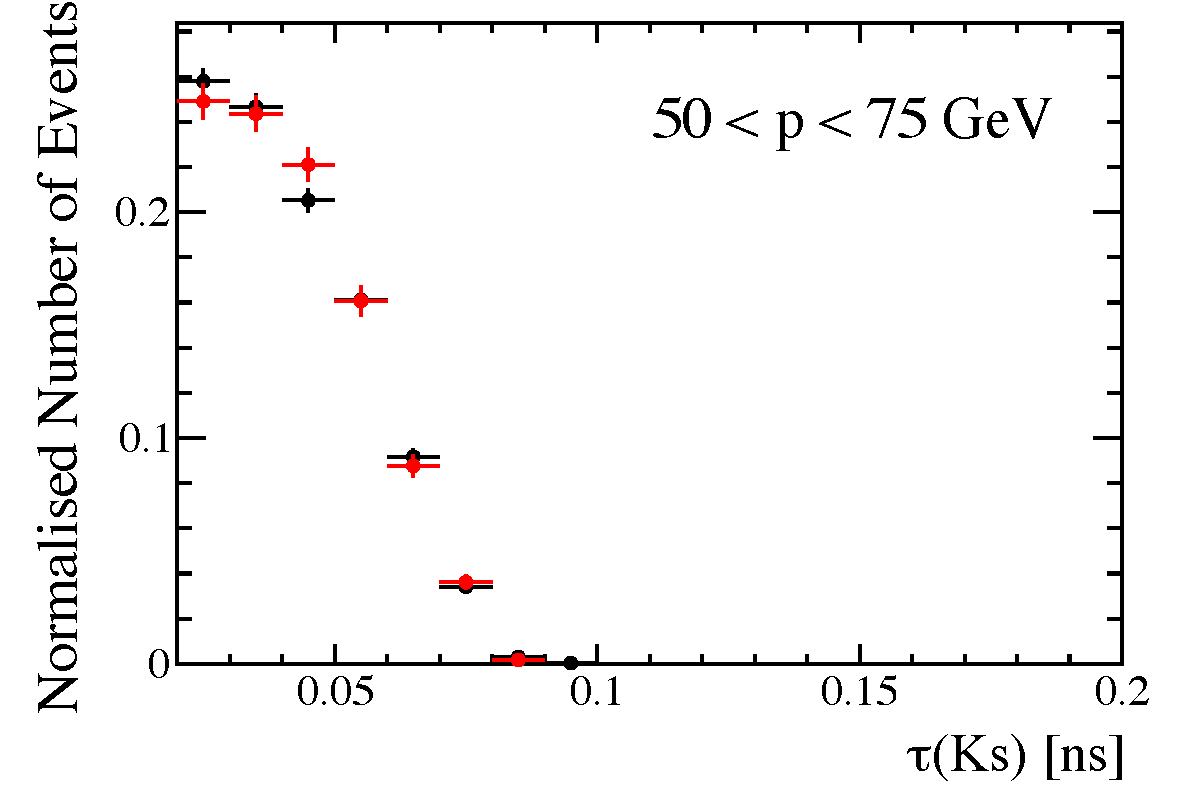
\includegraphics[width=0.48\textwidth]{jks_4}
    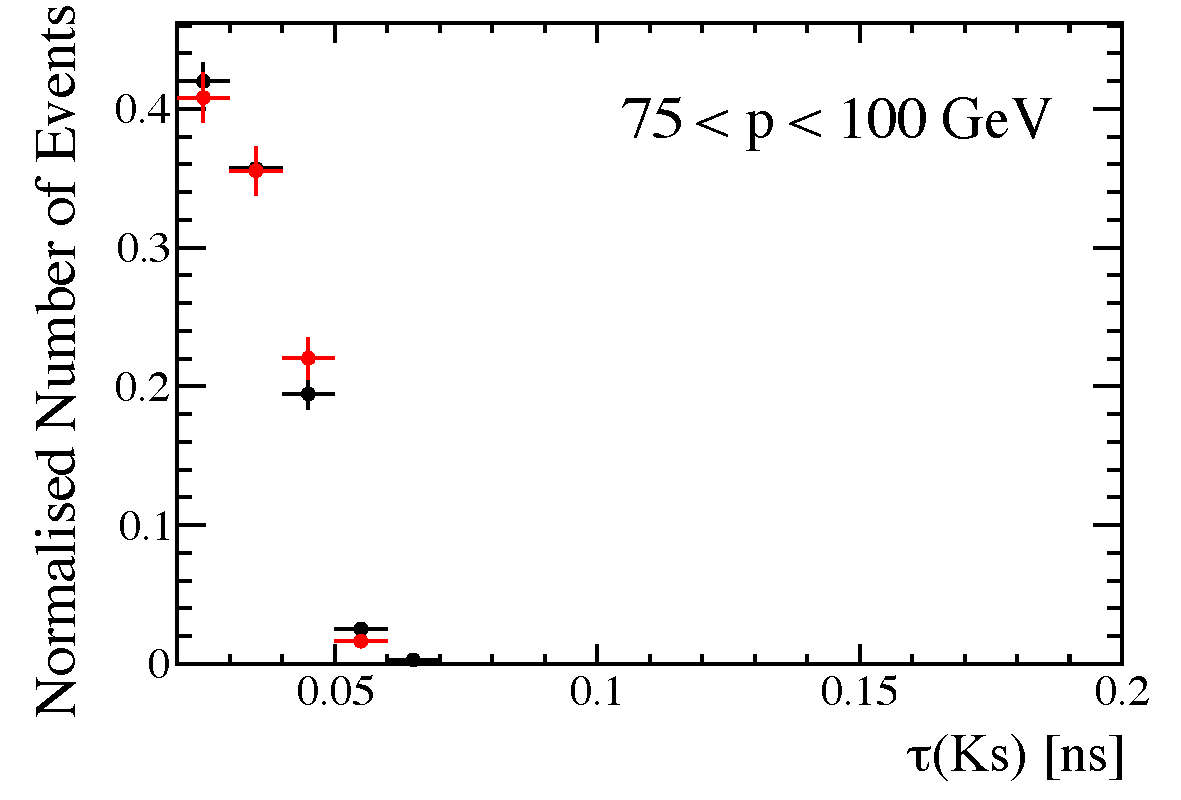
\includegraphics[width=0.48\textwidth]{jks_5}
    \caption[Validation of efficiency ratio at long lifetimes]
    {
      Reconstructed \KS lifetime distributions in bins of \KS momentum for (black) data and
      (red) simulation, where the \KS is part of the decay \decay{\Bd}{\jpsi\KS(\pipi)} and is a
      proxy \db candidate.
      Each plot is normalised to unit area.
      Good agreement is seen between the data and simulation.
    }
    \label{fig:db:syst:effrat}
  \end{center}
\end{figure}


Throughout the search it is assumed that the signal window, which extends $\pm2\sigma_m$ around
the test mass, contains $95\%$ of a total signal from a decaying \db.
A poorly modelled mass resolution will lead to an incorrect efficiency.
The accuracy of the mass resolution is tested using \btojpsikstr candidates falling within $60\mev$
of the nominal \Bd mass.
In actuality, it is observed that $94\%$ of \jpsitomumu candidates fall within $2\sigma_m$ of
the known \jpsi mass.
%Therefore a $1\%$ systematic uncertainty is applied.

%An important consideration is the spin of the \db.
%Since the spin of the \db is unknown, there are a range of possible angular distributions that may
%arise, each having a different detection efficiency.
%This can be studied using the angular acceptance models used in the \btokstrmumu angular
%analysis~\cite{LHCb-CONF-2015-002}.

\added{
The simulated events used to establish the efficiency for the \sm \btokstrmumu are generated
assuming true knowledge of the Wilson coefficients that contribute to the decay.
Results of the angular analysis of the decay \btokstrmumu from \lhcb, as described in
Ref.~\cite{LHCb-CONF-2015-002}, show that the Wilson coefficients used in the simulation are
consistent with those observed.
By generating an ensemble of toy simulated datasets, where the input Wilson coefficients for each
are varied randomly within their uncertainties.
The RMS deviation from this ensemble of toys with respect to the nominal value is assigned as the
systematic uncertainty from the mismodelling of the \sm \btokstrmumu channel, this is approximately
$1\%$.
}


%\deleted{
%The efficiency ratio $\varepsilon(\btokstrdb)/\varepsilon(\btokstrmumu)$ is approximately one, by
%construction, for each mass at zero lifetime.
%For larger lifetimes, the efficiency can be checked using data consistent with the decay
%\decay{\Bd}{\jpsi\KS}.
%It should be noted that in the displaced region a large uncertainty on the efficiency ratio will
%translate to a small uncertainty in the limits, because of the low statistics in that region.
%}
%
%\deleted{
%Studies undertaken in Ref.~\cite{Williams:2015xfa} show that the defining the boundary that separates
%the prompt and displaced regions to be $3\sigma_\tau$ is nearly optimal for any value of
%\lifetime{\db}.
%Only if $\tau_{\db}\simeq3\sigma_\tau$, then there may be some effect on the limits.
%The total effect of this must be demonstrated.
%}


\added{
The mismodelling of the lifetime resolutions is assessed using events consistent with the decay
\btojpsikstr in data.
Events falling in the displaced region, defined to be $\tau_{\mumu} > 3\sigma_\tau$, should
constitute $0.13\%$ of all events, but actually make up $(0.18\pm0.01)\%$.
To this end, a $3\%$ systematic uncertainty is applied, which is calculated by altering the
lifetime resolution as calculated using simulation until $0.18\%$ of events fell in the displaced
region.
}

\added{
The statistical uncertainty propagated from the normalisation yield is $5\%$.
As well as this, there is contamination from the $S$-wave component of the \Kstarz, which is
estimated to be $(4\pm4)\%$~\cite{LHCb-PAPER-2013-019}.
}

\added{
It has been noted that this analysis relies on the assumption that the background is smoothly
varying, and can be approximated as being locally linear.
This assumption clearly introduces an uncertainty, but this is already accounted for in the method
by the addition of the Gaussian, $\mathcal{G}(y, x, \sigma_y)$, in the likelihood shown in
\Eq{eq:db:like2}.
There is no need to add a systematic uncertainty for the chosen value of $\sigma_y$, because it is,
itself, an uncertainty and a maximal one.
It is also ensured that there is no variation between years and magnet polarity.
}












